\section{Домашнее задание}
\addcontentsline{toc}{section}{Домашнее задание}	% Добавляем его в оглавление

\begin{table} [htbp]
  \centering
  \begin{tabular}{| m{2.5cm} | m{1.5cm} | m{1.5cm} | m{1.5cm} | m{1.5cm} | m{1cm} | m{1cm} | m{1cm} | m{1.5cm}l |}
  \hline
  \multirow{2}{*}{ № варианта} &\multicolumn{4}{c|}{Исходные данные} &\multicolumn{4}{c}{Определяемые величины} &\\ \cline{2-10}
  &\centering $ R_1$, Ом &\centering $ C $, мкФ &\centering $ R_L $, Ом &\centering $ L $, Гн &\centering A &\centering B &\centering C &\centering C & \\
  \hline
  \centering \vspace{2mm} 1 \vspace{2mm} &\centering 100 &\centering 0,25 &\centering 100 &\centering 0,14 &\centering $ i_L(t) $ &\centering $ U_c(t) $ &\centering $ \tau $ &\centering $ T_c = \frac{2\pi}{\omega c}$ &\\
  \hline
  \end{tabular}
  \caption{Данные для расчета\label{tbl1}}
\end{table}


\begin{figure}[h]
\begin{minipage}[h]{0.45\linewidth}

\begin{center}
  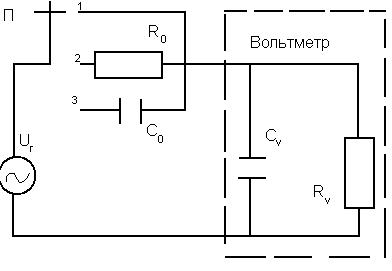
\includegraphics[width=1\linewidth]{scheme1}
  \caption{Исходная схема\label{sch1}}
\end{center}

\end{minipage}
\hfill
\begin{minipage}[h]{0.45\linewidth}

  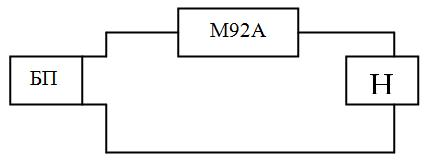
\includegraphics[width=1\linewidth]{scheme2}
  \caption{Схема сопротивлений\label{sch2}}

\end{minipage}
\end{figure}

Произведем расчет переходных процессов в цепи, показанной на рис.~\ref{sch1} классическим методом с учетом данных табл. \ref{tbl1}.

\begin{enumerate}

\item{Независимые начальные условия}

$ i_L(-0) = i_L(+0) = 0 $ A

$ u_C(-0) = u_C(+0) = 10 $ B

\item{Установившийся режим}

$ i_{L_{\text{у}}}(t) = 0 $ А

$ u_{C_{\text{у}}}(t) = E = 10 $ В 

\item{Поиск корней характеристического уравнения (рис.~\ref{sch2})}

$ R_1 + R_L + pL + \dfrac{1}{pC} = 0 $

$ 0,14p^2 + 200p + 4 \cdot 10^6 = 0 $

$ p_{1,2} = -1428,6 \pm 7423,08i $

\item{Искомые выражения имеют вид}
$$
	\left\{
		\begin{aligned}
			i_L(t) &= Ae^{-1428,6t}\sin(7423,08t + \varphi) \\
            u_C(t) &= E + Be^{-1428,6t}\sin(7423,08t + \psi) \\
			\dfrac{di_L}{dt} &= -1428,6Ae^{-1428,6t}\sin(7423,08t + \varphi) + 7423,08Ae^{-1428,6t}\cos(7428,08t + \varphi) \\
			\dfrac{du_C}{dt} &= -1428,6Be^{-1428,6t}\sin(7423,08t + \psi) + 7423,08Be^{-1428,6t}\cos(7428,08t + \psi) 			
        \end{aligned}
	\right.
$$

$$
	\left\{
		\begin{aligned}
			i_L(0+) &= A\sin(\varphi) = 0 \\
            u_C(0+) &= 10 + B\sin(\psi) = 0 \\
			\dfrac{di_L(0+)}{dt} &= -1428,6A\sin(\varphi) + 7423,08A\cos(\varphi) \\
			\dfrac{du_C(0+)}{dt} &= -1428,6B\sin(\psi) + 7423,08B\cos(\psi) 			
        \end{aligned}
	\right.
\hspace{5mm}
\Rightarrow
\hspace{5mm}
    \left\{
	\begin{aligned}
	  A &= 0,01 \\
      B &= 10,19 \\
      \varphi &= 0 \\
      \psi &= -79,1^{}
    \end{aligned}
	\right.
$$

$$
    \left\{
    \begin{aligned}
      i_L(t) &= 0,01e^{-1428,6t}\sin(7423,08t) \\
      \vspace{2mm}
      u_C(t) &= 10 + 10,19e^{-1428,6t}\sin(7423,08t - 79,1^{\circ})
    \end{aligned}
    \right.
$$

\vspace{2mm}
\begin{multicols}{2}
\begin{center}
  $ \tau = \bigg| \dfrac{1}{\delta} \bigg| = \dfrac{1}{1428,6} = 7 \cdot 10^{-4} $ (c)

\vspace{2mm}

  $ \Delta = e^{|\delta|T_{c}} = 3,35 $

  $ T_{c} = \dfrac{2\pi}{\omega_{c}} = \dfrac{6,28}{7423} = 8,5 \cdot 10^{-4} $ (c)

\vspace{2mm}

  $ \theta = | \delta |T_{c} = 1,214 $
\end{center}
\end{multicols}

\begin{figure}[h]
\begin{minipage}[h]{0.45\linewidth}

\begin{center}
  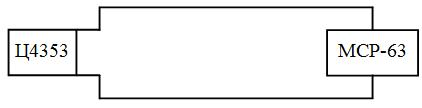
\includegraphics[width=1\linewidth]{scheme3}
  \caption{\label{sch3}}
\end{center}

\end{minipage}
\hfill
\begin{minipage}[h]{0.45\linewidth}

  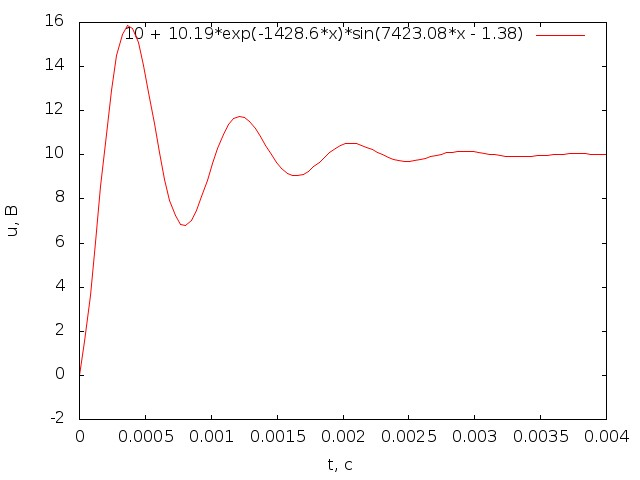
\includegraphics[width=1\linewidth]{scheme4}
  \caption{\label{sch4}}

\end{minipage}
\end{figure}

\end{enumerate}

\clearpage
